Por fim, queremos elaborar um pouco mais a dinâmica da tópico anterior(\ref{sec:secE}). 
Agora iremos impor uma fusão à um sólido. Para isso consideraremos um sistema de mesmas dimensões que o anterior 
e executaremos a dinâmica normalmente até atingir a cristalização como antes. A partir desse ponto
nosso impomos uma dinâmica externa às moléculas aumentando sua velocidade por um fator $\gamma = 1.5$. Repetimos 
essa dinâmica até que o sistema atinja um novo equilíbrio térmico. 

A imposição de novas velocidades é dada por 

\begin{equation}
    \mathbf{r}_{\text{anterior}} \longleftarrow \mathbf{r}_{\text{atual}} - (\mathbf{r}_{\text{atual}}-\mathbf{r}_{\text{anterior}})\gamma
    \label{eq:update_vels}
\end{equation}

Após muitas iterações e aplicando a (\ref{eq:update_vels}) às velocidades conseguimos observar a fusão acontecendo pela 
figura(\ref{fig:posicoes-finais-f}). Nota-se que talvez a escolha de intervalo para a figura do meio talvez não tenha sido 
tão boa, mas espero que seja possível perceber o inicio da difusão das moléculas em um entorno da cristalização anterior. 

\begin{figure}[h!]
    \centering
    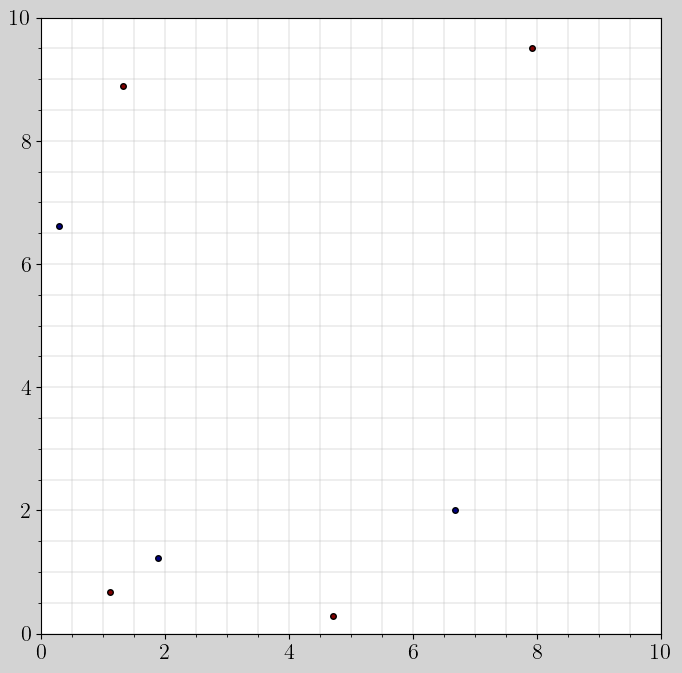
\includegraphics[width=0.95\linewidth]{tarefa-F/posicoes-finais.png}
    \caption{}
    \label{fig:posicoes-finais-f}
\end{figure}


E para finalizar, também foi feito um gráfico da energia desse sistema. Era de se esperar que fosse haver um 
aumentando de energia simplesmente pelo fato de ser um processo de fusão e o gráfico abaixo (\ref{fig:energia-f})
expressa esse fato assim como mostra o quão abrupto é o aumento dessa energia, já que a nossa dinâmica 
de aumento velocidades é instantâneo.

\begin{figure}[h!]
    \centering
    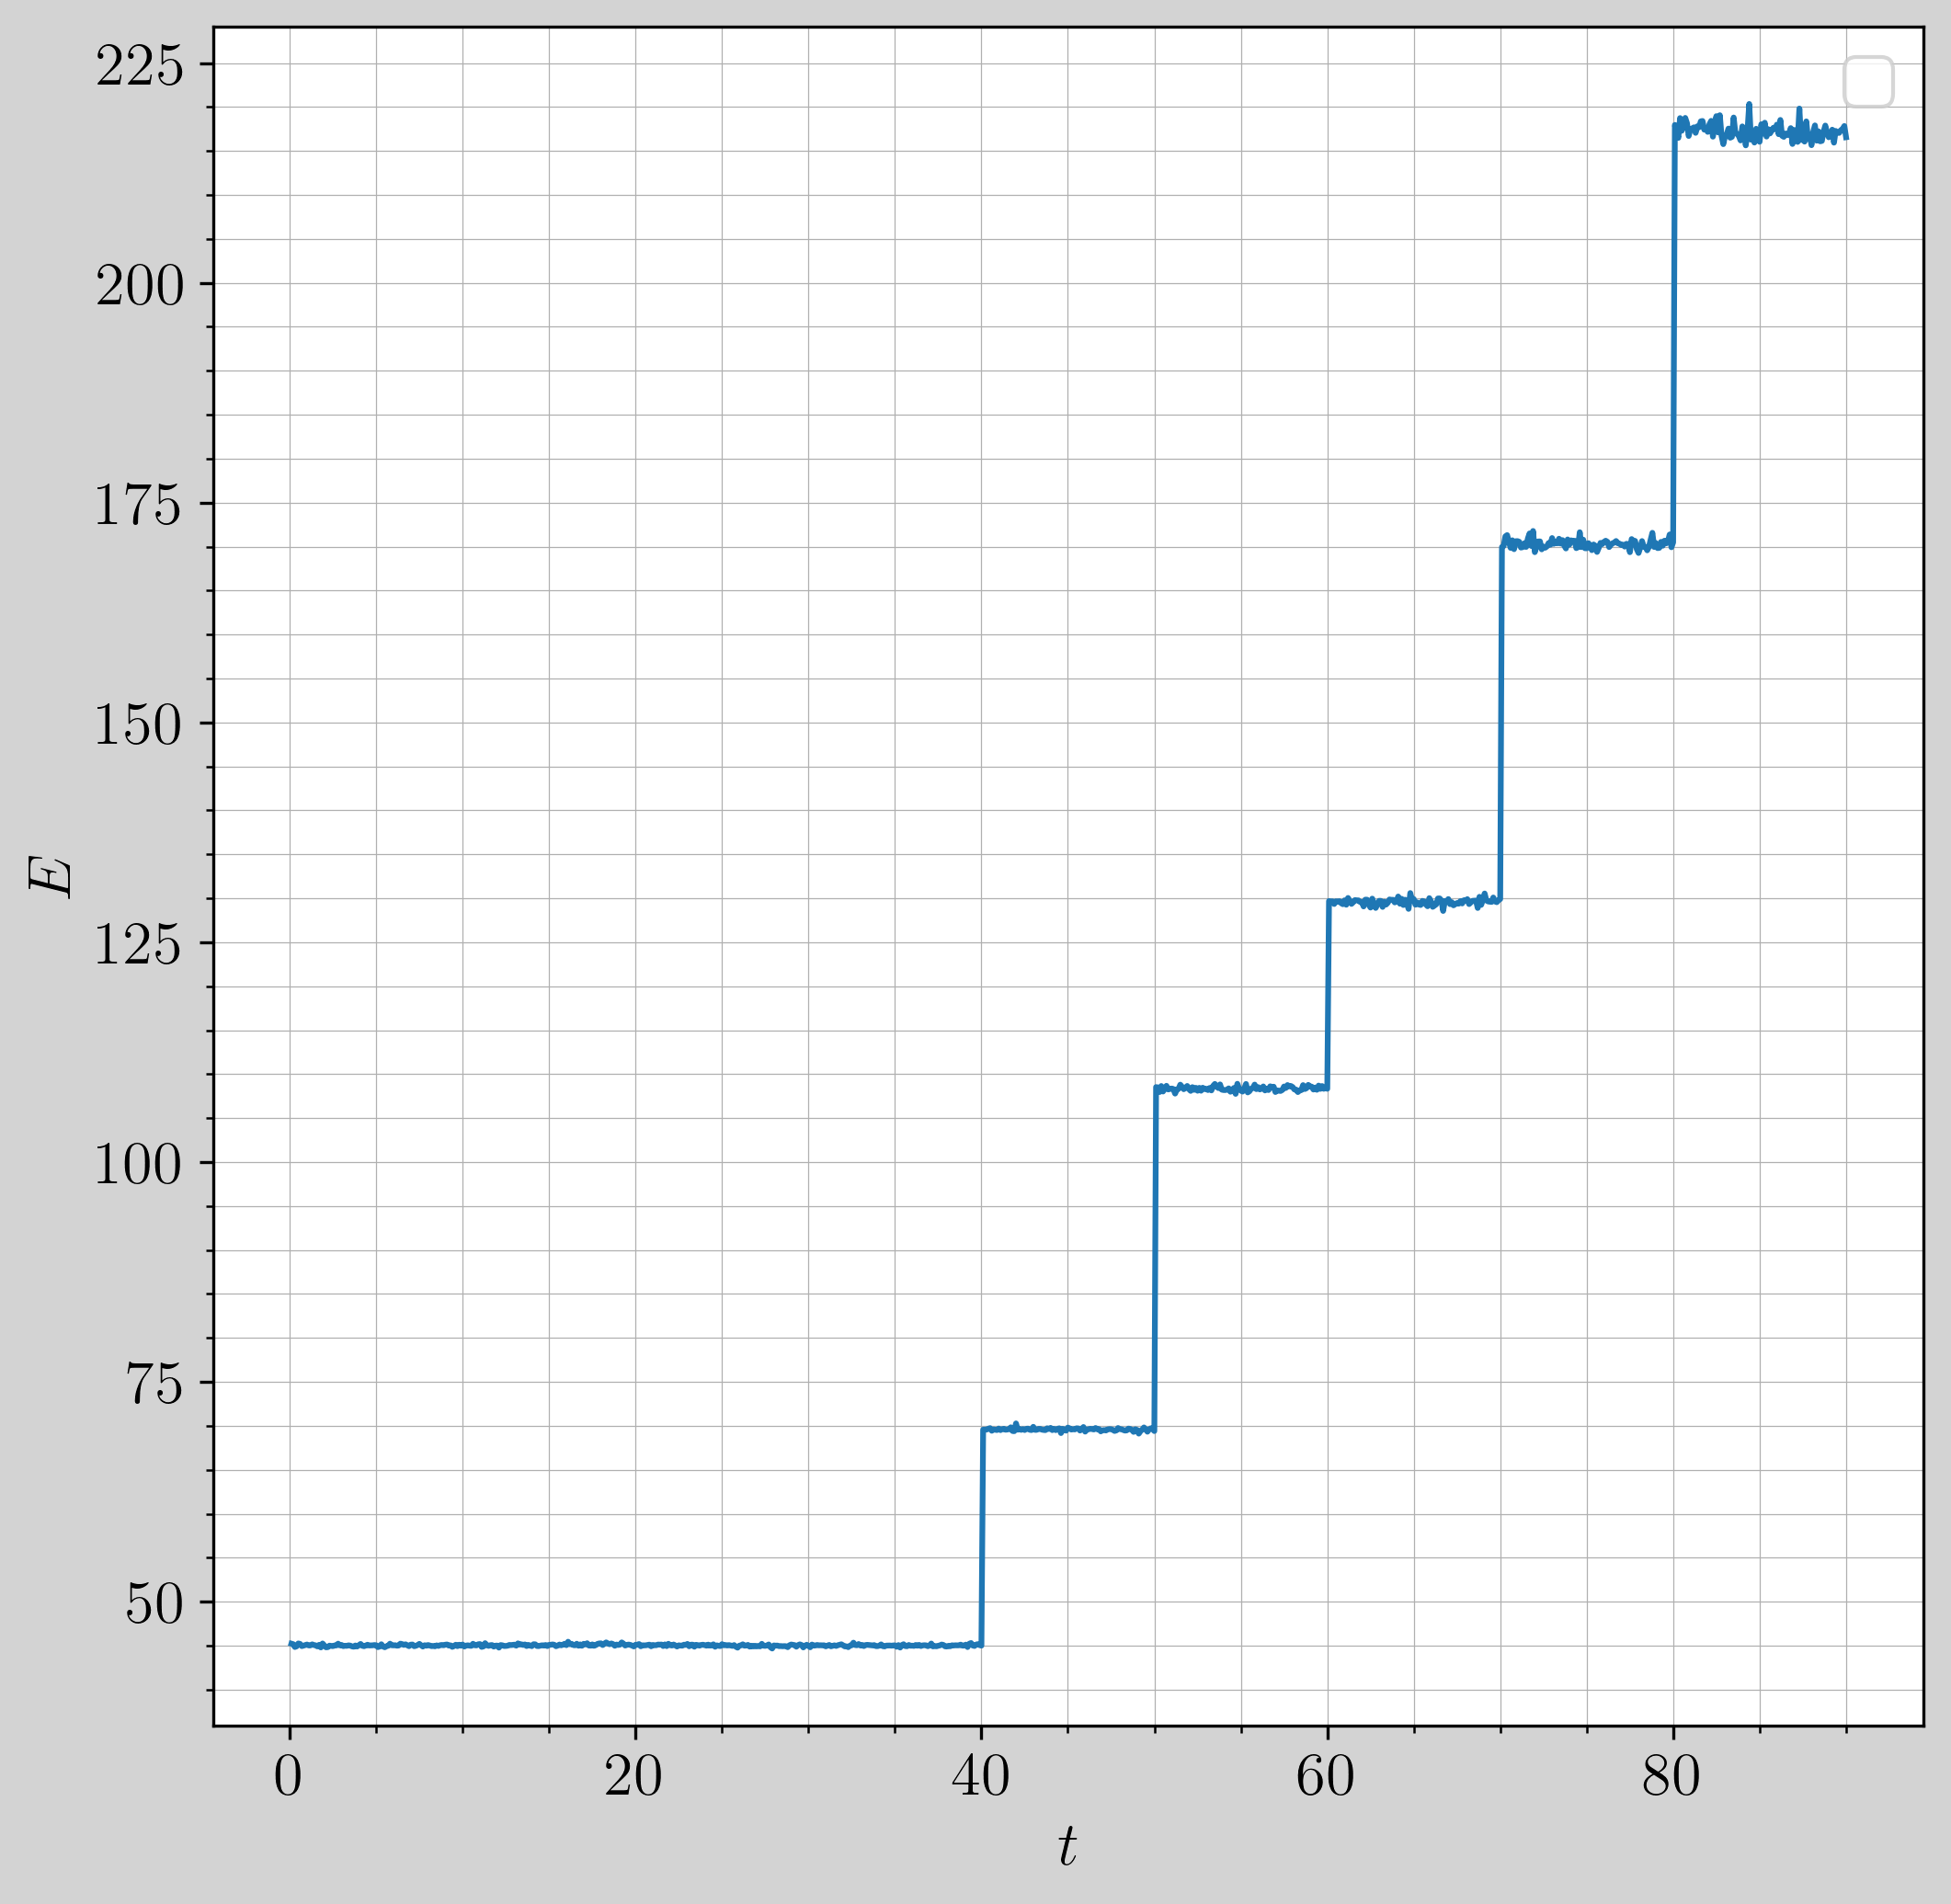
\includegraphics[width=0.4\linewidth]{tarefa-F/energia.png}
    \caption{Energia total a cada tempo.}
    \label{fig:energia-f}
\end{figure}


\clearpage
\subsection{Implementação - Simulação F}
Um detalhe que não consegui explicar sobre essa simulação é que a única forma que consegui fazer a fusão acontecer 
corretamente foi considerando apenas uma das componenentes na (\ref{eq:update_vels}) e não todo vetor. 

\begin{minted}{fortran}
    ! Tarefa F 
    implicit real*8(a-h, o-y)
    parameter (pi = acos(-1.e0))
    dimension r_prev(20, 2)
    dimension r_curr(20, 2)
    dimension r_next(20, 2)
    dimension v(20, 2)
    dimension acc(2)
    dimension r(20, 20)


    ! TAREFA F 
    open(unit=85, file="saidas/tarefa-F/parametros.dat")
    open(unit=86, file="saidas/tarefa-F/posicoes-iniciais.dat")
    open(unit=87, file="saidas/tarefa-F/evolucao-posicoes-1.dat")
    open(unit=88, file="saidas/tarefa-F/evolucao-posicoes-2.dat")
    open(unit=89, file="saidas/tarefa-F/evolucao-posicoes-3.dat")
    open(unit=90, file="saidas/tarefa-F/energia.dat")

    ! Reset variables: 
    r_prev = 0
    r_curr = 0
    r_next = 0
    v = 0

    L = 4
    rL = 4d0
    N = 16

    dt = 5e-3
    v0 = 0.2

    write(85, *) N, L, v0, dt 
    close(85)

    ! Initialize particles 

    n_cols = ceiling(sqrt(N*1d0))
    n_rows = ceiling((N*1d0)/(n_cols*1d0)) 
    
    ! Spacing 1/4 
    x_spacing = L/(1d0*n_cols)
    y_spacing = L/(1d0*n_rows)
    spacing = min(x_spacing, y_spacing)/4.0 
    
    ! Centering in the grid
    x_offset = x_spacing / 2.0 
    y_offset = y_spacing / 2.0
    
    call srand(3512341)

    k = 1 
    do j = 1, n_rows 
          do i = 1, n_cols 
                r_curr(k, 1) = (i-1)*x_spacing+x_offset
                r_curr(k, 2) = (j-1)*y_spacing+y_offset
                
                r_curr(k, 1) = r_curr(k,1)+(rand())*spacing
                r_curr(k, 2) = r_curr(k,2)+(rand())*spacing
                
                theta = 2*pi*rand()
                
                v(k, 1) = v0*cos(theta)
                v(k, 2) = v0*sin(theta)
                
                r_prev(k, 1) = r_curr(k, 1) - v(k, 1) * dt 
                r_prev(k, 2) = r_curr(k, 2) - v(k, 2) * dt 
                k=k+1
          end do 
    end do

    do i = 1, N 
          write(76, *) r_curr(i, 1), r_curr(i, 2)
    end do 
    close(76)

    ! Dynamics 
    do k = 1, 18000 
          t = k * dt 
          acc(1) = 0d0 
          acc(2) = 0d0

          E_k = 0d0
          U = 0d0

          do i = 1, N 
                acc(1) = 0d0 
                acc(2) = 0d0
                do j = 1, N 
                      if(i /= j) then
                           call compute_acc(N,i,j,L,r_curr,acc, r)
                      end if
                end do 
                ! UPDATE POSITIONS
                r_next(i,1) = 2*r_curr(i,1)-r_prev(i,1)+acc(1)*(dt**2)
                r_next(i,2) = 2*r_curr(i,2)-r_prev(i,2)+acc(2)*(dt**2) 

                ! APPLY PBC
                r_next(i,1) = mod(r_next(i,1)+rL, rL)
                r_next(i,2) = mod(r_next(i,2)+rL, rL)

                delta_r_x = delta_pbc(r_next(i,1),r_prev(i,1),L)
                delta_r_y = delta_pbc(r_next(i,2),r_prev(i,2),L)

                ! UPDATE VELOCITIES using adjusted displacements
                v(i, 1) = delta_r_x / (2 * dt)
                v(i, 2) = delta_r_y / (2 * dt)

          end do

          r_prev(:, 1) = r_curr(:, 1)
          r_prev(:, 2) = r_curr(:, 2)
          
          r_curr(:, 1) = r_next(:, 1)
          r_curr(:, 2) = r_next(:, 2)

          if(mod(k, 20) == 0) then 
                if(k > 16000) then
                      ! Liquid end 
                      do i = 1, N
                            write(89,*) k, r_curr(i,1),r_curr(i,2)
                      end do
                else if (k > 10000 .and. k < 12000) then
                      !  Liquit initial
                      do i = 1, N 
                            write(88,*) k, r_curr(i,1),r_curr(i,2)
                      end do
                else if (k > 2600 .and. k < 3200) then 
                      ! Crystal
                      do i = 1, N 
                            write(87,*) k, r_curr(i,1),r_curr(i,2)
                      end do
                end if 

          end if

          ! Increase velocity
          if(mod(k, 2000) == 0 .and. k > 7000) then
                do i = 1, N
                r_prev(i,1)=r_curr(i,1)-(r_curr(i,1)-r_prev(i,1))*1.5
                end do
          end if

          if (mod(k,20) == 0) then
                E = 0d0
                call compute_energy(N, L, v, r_curr, E, r)
                write(90,*) k, E
          end if
    end do 
    close(85)
    close(86)
    close(87)
    close(88)
    close(89)
    close(90)
    end
    ! Submodules for molecular dynamic simulations
    ! Velocity delta 
    function delta_pbc(r_next, r_prev,L)
          implicit real*8(a-h, o-y)
          delta_pbc = r_next - r_prev
          delta_pbc = delta_pbc - L * nint(delta_pbc / L)
    end function delta_pbc

    subroutine initialize_particles(N, L, r_curr,r_prev, v, v0)
          implicit real*8(a-h, o-y)
          dimension r_prev(20, 2)
          dimension r_curr(20, 2)
          dimension v(20, 2)
         
          ! Defining # rows/columns 
          n_cols = ceiling(sqrt(N*1d0))
          n_rows = ceiling((N*1d0)/(n_cols*1d0)) 
          
          ! Spacing 1/4 
          x_spacing = L/(1d0*n_cols)
          y_spacing = L/(1d0*n_rows)
          spacing = min(x_spacing, y_spacing)/4.0 
          
          ! Centering in the grid
          x_offset = x_spacing / 2.0 
          y_offset = y_spacing / 2.0
          call srand(562369)

          k = 1 
          do j = 1, n_rows 
                do i = 1, n_cols 
                      r_curr(k, 1) = (i-1)*x_spacing+x_offset
                      r_curr(k, 2) = (j-1)*y_spacing+y_offset
                      
                      r_curr(k, 1) = r_curr(k,1)+(rand())*spacing
                      r_curr(k, 2) = r_curr(k,2)+(rand())*spacing

                      theta = 2*pi*rand()
                      v(k, 1) = v0*cos(theta)
                      v(k, 2) = v0*sin(theta)
                      
                      r_prev(k, 1) = r_curr(k, 1) - v(k, 1) * dt 
                      r_prev(k, 2) = r_curr(k, 2) - v(k, 2) * dt 
                      k=k+1
                end do 
          end do
    end subroutine initialize_particles

    ! Updates acceleration a = ax, ay 
    ! between particle i and all others
    subroutine compute_acc(N,i,j,L,r_curr,acc, r)
          implicit real*8(a-h, o-y)
          dimension r_curr(20, 2)
          dimension acc(2)
          dimension r(20, 20)
          epsilon = 1e-3

          dx = r_curr(i, 1) - r_curr(j, 1)
          dy = r_curr(i, 2) - r_curr(j, 2)

          dx = dx - L * nint(dx / L)
          dy = dy - L * nint(dy / L)

          r_ij = sqrt(dx**2 + dy**2)
          
          r(i, j) = r_ij 
          r(j, i) = r_ij

          if(r_ij > epsilon .and. r_ij <= 3d0) then 
                F = 24.0 * (2d0/r_ij**13 - 1d0/r_ij**7)
                acc(1) = acc(1) + F * dx / r_ij 
                acc(2) = acc(2) + F * dy / r_ij
          end if 
    end subroutine compute_acc

    subroutine compute_energy(N, L, v, r_curr, E, r)
          implicit real*8(a-h, o-y)
          dimension v(20, 2)
          dimension r_curr(20, 2)
          dimension r(20, 20)
          
          epsilon = 1e-3
          Tk = 0d0
          do i = 1, N
              Tk = Tk + 0.5 * (v(i, 1)**2 + v(i, 2)**2)
          end do
          U = 0d0
          do i = 1, N
            do j = i + 1, N
                r_ij = r(i, j)

                if (r_ij > epsilon .and. r_ij <= 3d0) then
                    U = U + 4 * (r_ij**(-12) - r_ij**(-6))
                end if
            end do
          end do
          E = Tk + U
    end subroutine compute_energy
\end{minted}